\section{Bitmap}

\subsection{Aperçu du Bitmap}
Le format BITMAP aussi appelé DIB (Device Independent Bitmap) a été conçu par Windows corporation pour pouvoir échanger des images entre devices sans avoir à se soucier de la logique de ceux-ci.
Ces images ont des extensions .bmp ou encore .dib.\\
Une image bitmap est un format de fichier généralement non compressé. Cela signifie que chaque pixel possède sa représentation sous forme d'une série de bits.
Les bitmaps n'ont aucune perte de données et sont donc généralement plus lourds.
On peut opposer leur structure à celle d'une image PNG, JPEG ou encore GIF, qui utilisent la compression pour regrouper des pixels similaires.\\
Les headers des bitmaps peuvent employer plusieurs versions. Ces versions donnent plus ou moins de métadonnées sur le bitmap. 
Le BITMAPINFOHEADER est une des versions les plus simples et rétrocompatible. 
Actuellement, il existe des versions plus complètes, tels que le BITMAPV4HEADER ou BITMAPV5HEADER.\\
La structure du format BITMAP est connue et disponible en ligne. En voici un schéma, utilisant le BITMAPINFOHEADER :\\

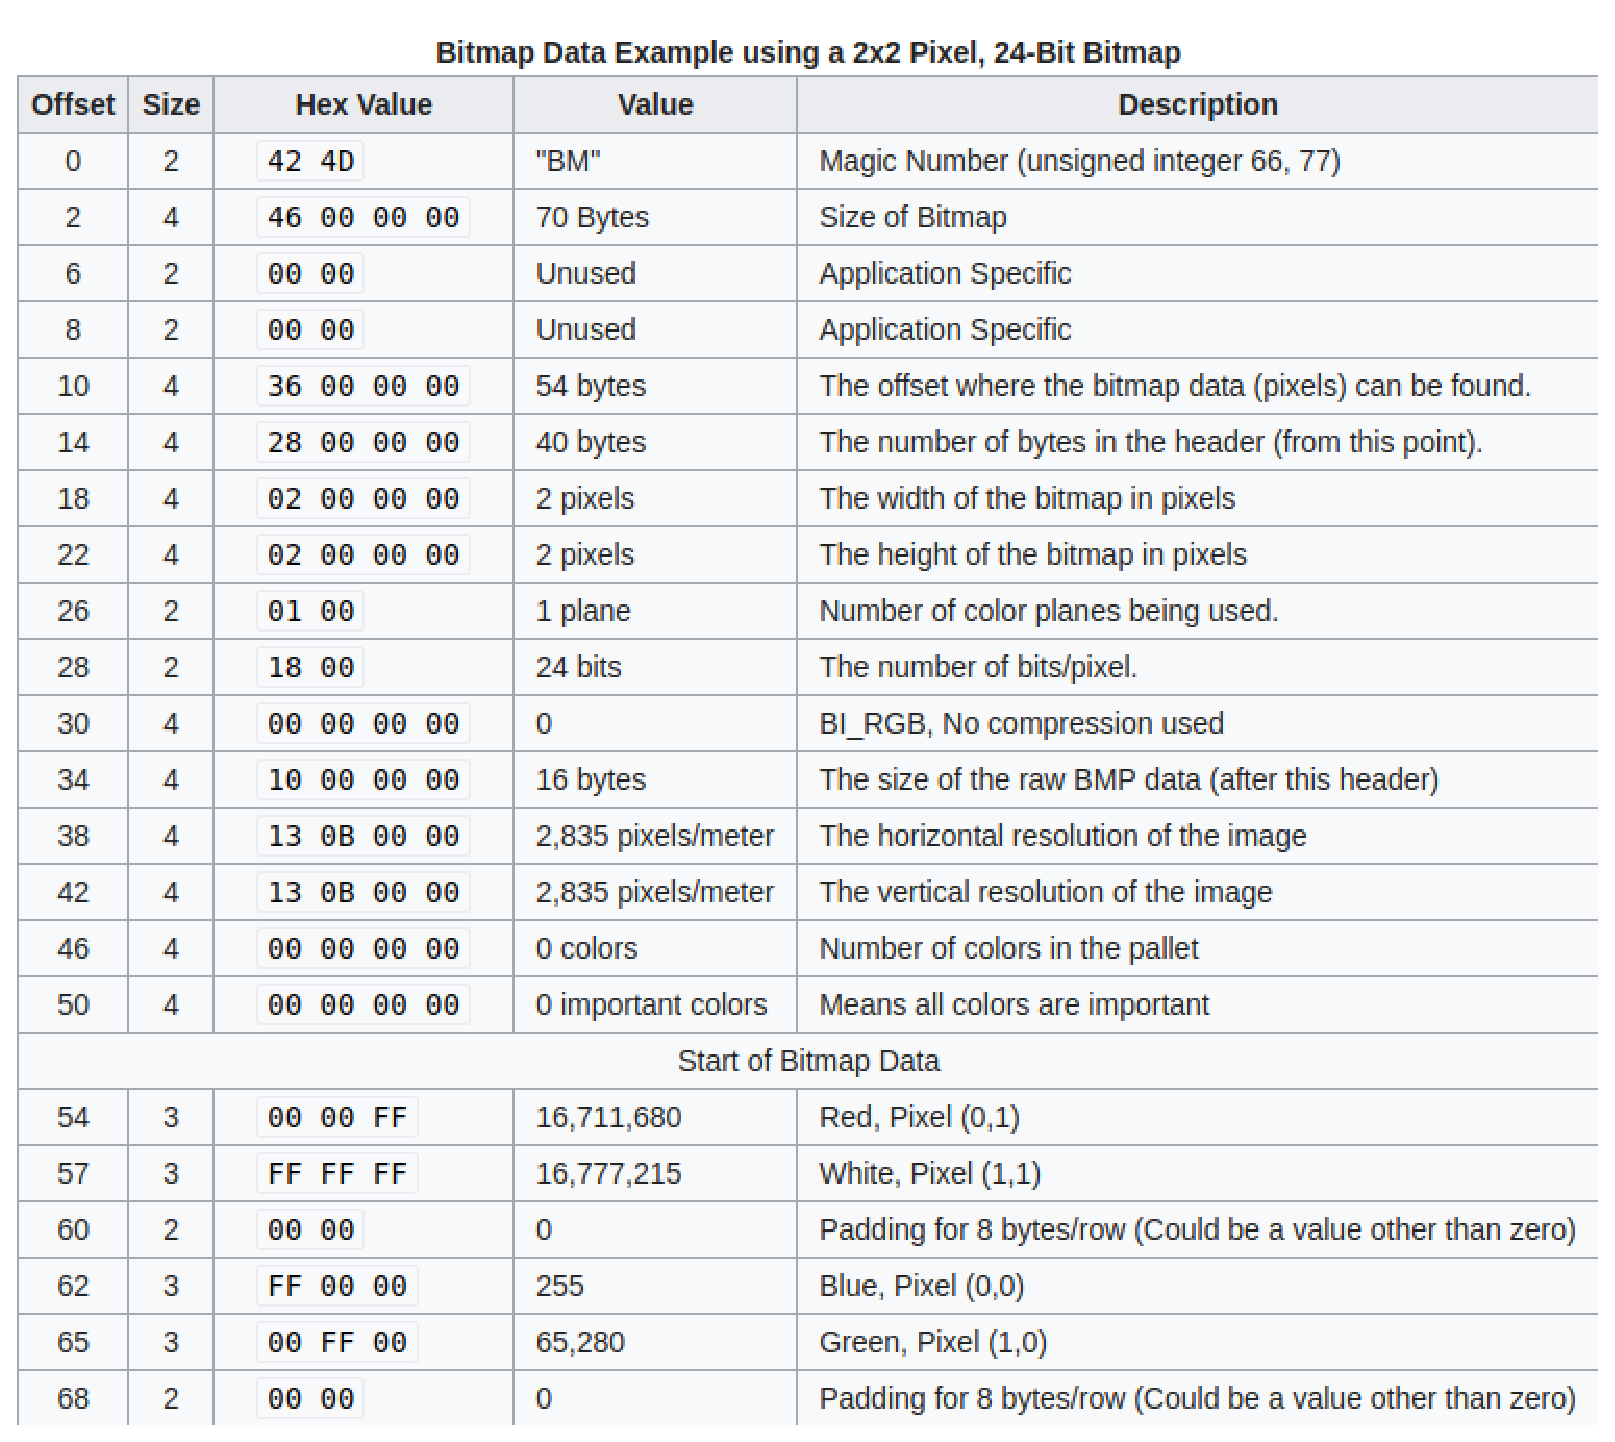
\includegraphics[width=14cm]{bitmap_structure.eps}

\subsection{Application du LSB}
Nous cachons les données dans les bytes décrivant les couleurs de l'image source, juste après le header.
Les modifications étant faites sur des couleurs, l'image est peu altérée. Les modifications sont invisibles à l'oeil humain.
De plus, ce fichier n'utilisant généralement pas d'algorithme de compression, on ne doit pas se soucier de perte de données, 
ce qui aurait probablement impacter le décodage d'une image dans laquelle on aurait caché des données.

\vspace{1.5cm}
